\documentclass[a4paper,8pt,twocolumn]{article}
\usepackage[UTF8]{ctex}
\usepackage{graphicx}
\usepackage{fancyhdr}
\usepackage{amsmath}
\usepackage{subcaption}
\usepackage{float}
\usepackage[
  left=2cm,
  right=2cm,
  top=1.5cm,
  bottom=2.5cm
]{geometry}
\usepackage{siunitx}
\usepackage{booktabs}
\usepackage{enumitem}
\usepackage{array}
\usepackage{tabularx}
\newcolumntype{Y}{>{\centering\arraybackslash}X}
\usepackage{amssymb}

\sisetup{
  per-mode=symbol,
  separate-uncertainty = true
}

\title{
  \textbf{\huge RX2：基于LabVIEW的PID控温设计实验}
}
\author{
  黄雨~24352027\\
  \small 中山大学物理学院~广东~广州
}

\pagestyle{fancy}
\fancyhf{}
\fancyhead[C]{RX2：基于LabVIEW的PID控温设计实验}
\fancyfoot[C]{\thepage}

\begin{document}
\maketitle
\newpage

%%%%%%%%%%%%%%%%%%%%%%%%%%%%%%%%%%%%%%%%%%%%%%%%%%%%%%%%%%%%
\section{实验目的}

\begin{enumerate}
  \item 掌握用LabVIEW控制可编程直流稳压电源的方法；
  \item 建立基于LabVIEW的温度控制系统，理解自动化控制的基本思想和方法；
  \item 利用PID控制等方案实现电阻控温，熟悉控制参数调节的基本方法。
\end{enumerate}

%%%%%%%%%%%%%%%%%%%%%%%%%%%%%%%%%%%%%%%%%%%%%%%%%%%%%%%%%%%%
\section{实验仪器与装置}

\begin{itemize}
  \item 实验测控用计算机（安装了NI LabVIEW软件和可编程电源驱动程序）；
  \item Rigol DP802A可编程直流电源；
  \item NI CompactDAQ单槽机箱和NI\,9211数据采集器；
  \item 导线、电阻、热电偶等。
\end{itemize}

%%%%%%%%%%%%%%%%%%%%%%%%%%%%%%%%%%%%%%%%%%%%%%%%%%%%%%%%%%%%
\section{实验原理}

\subsection{自动控制系统}

自动控制是指在无人直接干预下，利用物理装置对被控对象进行合理控制，使被控量保持恒定或按一定规律变化的过程。典型的闭环控制系统包括控制器、被控对象和检测装置，对其基本要求是\textbf{稳定、快速、准确}。

开环控制结构简单、容易稳定，但由于缺乏反馈，控制精度较差；闭环控制通过反馈量与给定量的比较产生偏差，由控制器动态调节控制量，可有效抑制扰动、提高精度，但参数不当时可能出现超调、振荡甚至发散。

\subsection{PID控制原理}

PID控制器的输出由比例(P)、积分(I)和微分(D)三项加权组合而成：
\begin{equation}
  u(t)=K_p\!\left[e(t)+\frac{1}{T_i}\int_0^t e(\tau)\,\mathrm{d}\tau
       +T_d\,\frac{\mathrm{d}e(t)}{\mathrm{d}t}\right]
  \tag{RX2.1}
\end{equation}
其中$e(t)$为设定值与反馈值之差，$K_p$为比例增益，$T_i$为积分时间常数，$T_d$为微分时间常数。

\begin{itemize}
  \item \textbf{比例控制}（$K_p$）：反映偏差的实时响应，$K_p$越大响应越快，但过大会引起超调或振荡，且纯比例控制可能存在稳态误差；
  \item \textbf{积分控制}（$T_i$）：累积偏差以消除稳态误差，但可能引入积分饱和；
  \item \textbf{微分控制}（$T_d$）：预判偏差变化趋势，抑制超调、起"刹车"作用，但可能放大高频噪声。
\end{itemize}

\subsection{电阻温度的传递函数模型}

假设电阻内部温度均匀（集总参数法），以单一温度$T$描述其表面温度，有
\begin{equation}
  \rho V C_p\,\frac{\mathrm{d}T}{\mathrm{d}t}
    =hA(T_e-T)+Q
  \tag{RX2.2}
\end{equation}
其中$\rho V C_p$为电阻总热容，$hA$为表面整体换热系数，$T_e$为环境温度，$Q=I^2R$为焦耳热。

引入$\theta=T-T_e$，令$\tau=\rho V C_p/(hA)$，$q=Q/(\rho V C_p)$，经Laplace变换得传递函数
\begin{equation}
  \frac{\theta(s)}{q(s)}=\frac{\tau}{1+\tau s}
  \tag{RX2.3}
\end{equation}

在P控制器（增益$K_p$）作用下，闭环传递函数为
\begin{equation}
  \frac{\theta(s)}{r(s)}=\frac{K_p\tau/(1+K_p\tau)}{1+\tau s/(1+K_p\tau)}
  \tag{RX2.4}
\end{equation}
可见P控制使系统时间常数由$\tau$缩短为$\tau/(1+K_p\tau)$，加快了系统响应。

%%%%%%%%%%%%%%%%%%%%%%%%%%%%%%%%%%%%%%%%%%%%%%%%%%%%%%%%%%%%
\section{实验内容与步骤}

\subsection{用LabVIEW控制Rigol直流稳压电源}

\begin{enumerate}[label=(\alph*)]
  \item 连接实验装置：可编程电源通过USB控制线接计算机，CH1输出接电阻两端；热电偶探头贴于电阻表面，热电势信号端接NI\,9211模块的ai0通道（注意正负极）。
  \item 用NI MAX软件检查数据采集器和可编程电源是否正确连接。
  \item 用LabVIEW编写可编程电源驱动程序（图\,\ref{fig:circle1}），测试温度读取与电阻加热功能。
  \item 用$5\sim\SI{10}{V}$测试不同加热功率下的升温和降温曲线，估计电阻的热容和对流换热情况。
  \item 记录电压为$\SI{10}{V}$时电阻升温的最高温度$T_{\max}$及室温$T_e$。
\end{enumerate}

\begin{figure}[H]
  \centering
  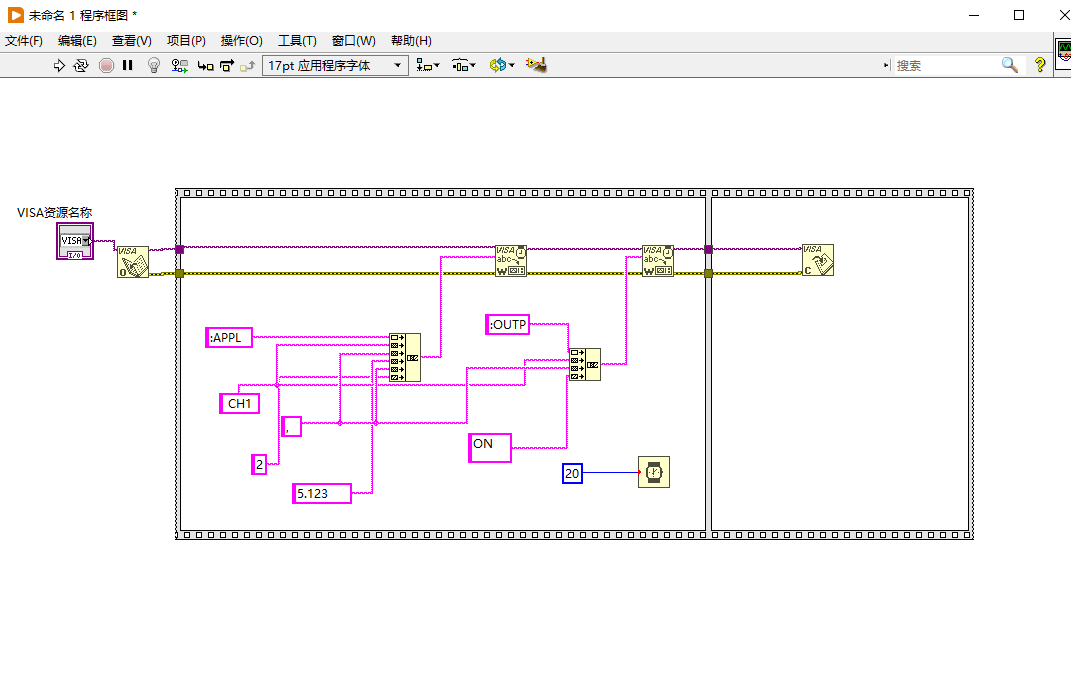
\includegraphics[width=0.95\columnwidth]{Circle_1.png}
  \caption{LabVIEW控制Rigol直流稳压电源程序框图}
  \label{fig:circle1}
\end{figure}

\subsection{PID控制调参}

\begin{enumerate}[label=(\alph*)]
  \item 在LabVIEW程序中加入PID控制器模块，按闭环控制结构编写程序（图\,\ref{fig:circle2}）。
  \item 调试设定温度$T_1=(T_{\max}+T_e)/2$，分别改变$(K_c,\,T_i,\,T_d)$参数，观测控温效果，寻找响应最快、超调最小的参数组合。
  \item 按教师现场提供的四个设定温度，记录设定温度曲线与实际温度曲线，评估不同PID参数下的控温效果。
\end{enumerate}

\begin{figure}[H]
  \centering
  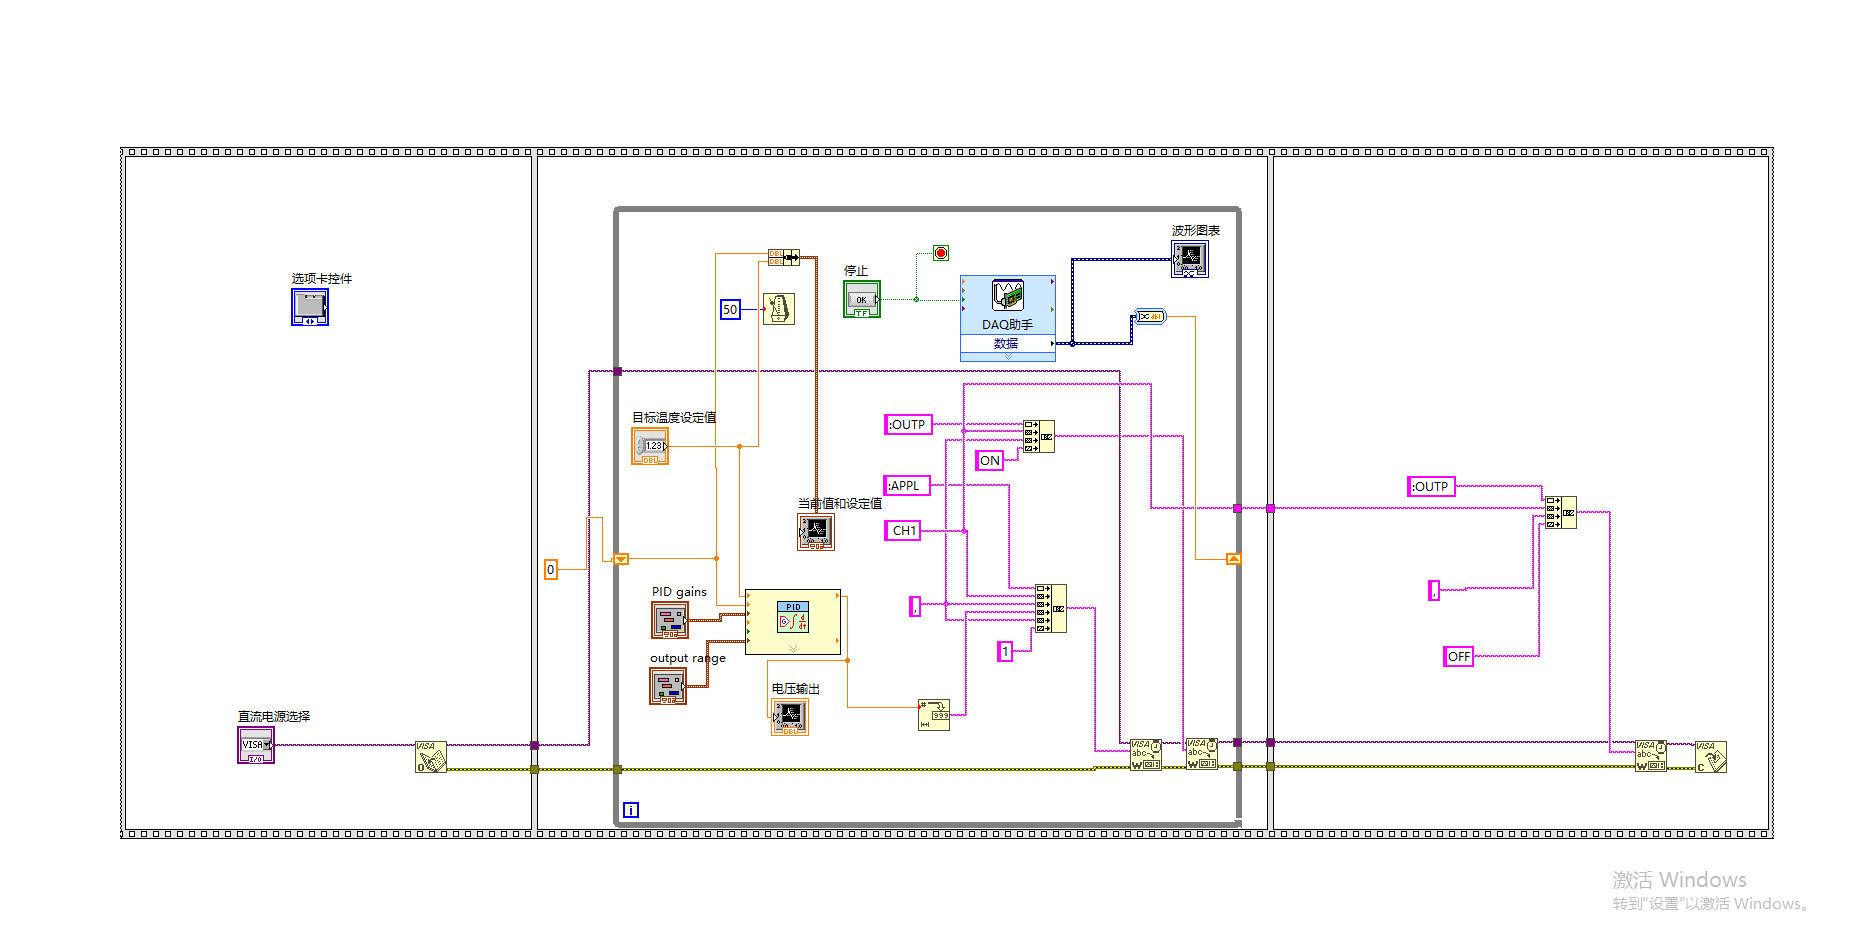
\includegraphics[width=0.95\columnwidth]{Circle_2.png}
  \caption{PID控制调参程序框图}
  \label{fig:circle2}
\end{figure}

%%%%%%%%%%%%%%%%%%%%%%%%%%%%%%%%%%%%%%%%%%%%%%%%%%%%%%%%%%%%
\section{实验结果与分析}
\label{sec:results}

\subsection{基本参数测量}

在$\SI{10}{V}$加热电压下测得：
\begin{itemize}
  \item 电阻升温最高温度：$T_{\max}=\SI{68.7}{\degreeCelsius}$
  \item 室温：$T_e=\SI{27.7}{\degreeCelsius}$
  \item 调试设定温度：$T_1=(T_{\max}+T_e)/2=(68.7+27.7)/2=\SI{48.2}{\degreeCelsius}$
\end{itemize}

\subsection{升温与降温曲线及热参数估计}

\subsubsection{实验曲线}

图\,\ref{fig:heatcool}给出了在$5\sim\SI{10}{V}$六组加热电压下，电阻从室温出发的升温曲线（$0\sim\SI{180}{s}$）和断电后的自然降温曲线（$\SI{180}{s}\sim\SI{360}{s}$）。室温$T_e=\SI{25.6}{\degreeCelsius}$。

\begin{figure*}[ht]
  \centering
  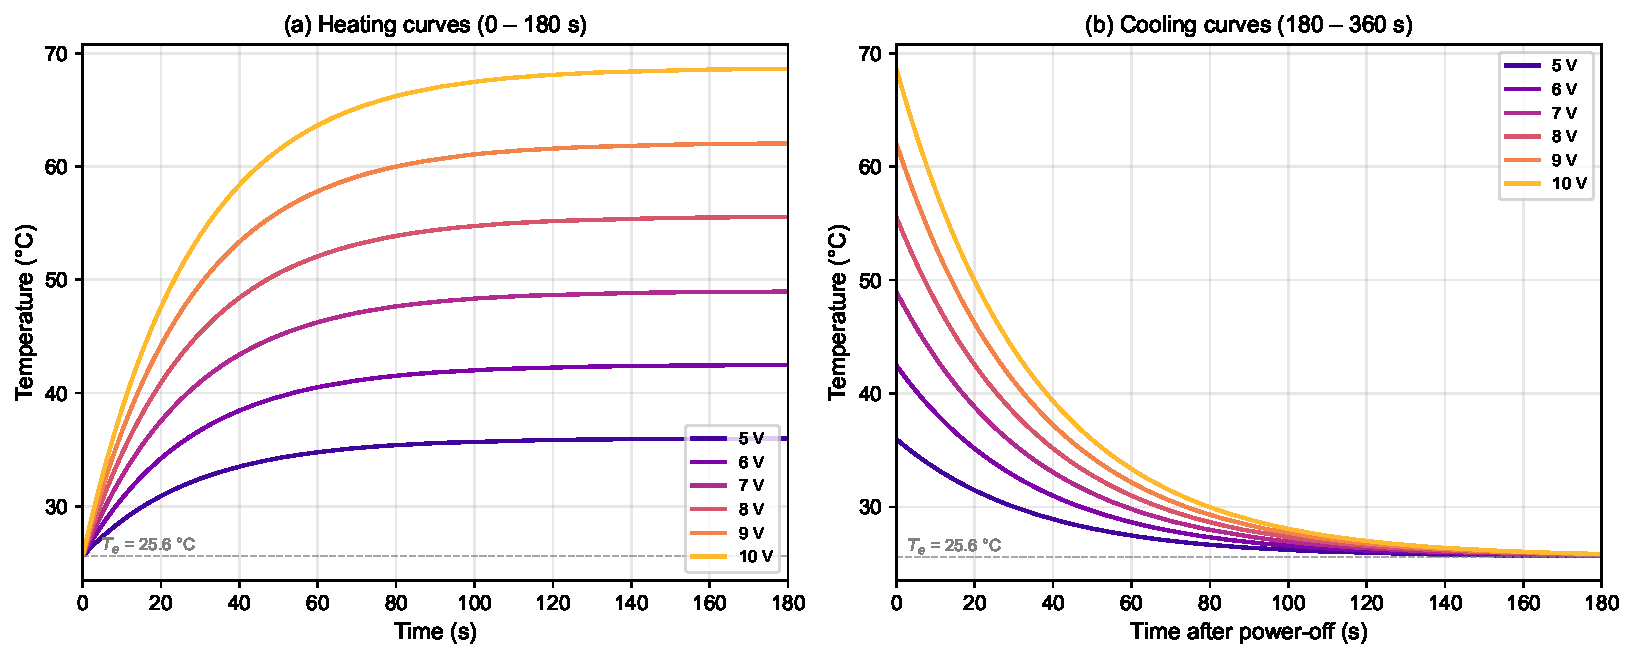
\includegraphics[width=\textwidth]{fig_heat_cool.pdf}
  \caption{不同加热电压下的升温曲线（左）与降温曲线（右）。$t=\SI{180}{s}$时断电。}
  \label{fig:heatcool}
\end{figure*}

从图中可见：加热电压越高，升温速率越快，稳态温度越高；断电后各曲线以相似的指数形式衰减回室温，反映了系统具有统一的热时间常数。

\subsubsection{热模型与参数提取}

根据集总参数热模型（式\,RX2.2），令$\theta=T-T_e$，加热阶段（$Q=V^2/R=\text{const}$）的解为
\begin{equation}
  \theta(t)=\Delta T_\infty\!\left(1-e^{-t/\tau}\right),\quad
  \Delta T_\infty=\frac{V^2}{RhA}
  \tag{RX2.5}
\end{equation}
断电后降温阶段（$Q=0$）为
\begin{equation}
  \theta(t)=\theta_\text{peak}\,e^{-(t-t_0)/\tau}
  \tag{RX2.6}
\end{equation}
两阶段共享同一时间常数$\tau=\rho V C_p/(hA)$。

对六组降温曲线分别进行指数拟合，得到的时间常数高度一致（图\,\ref{fig:ssfit}左示$\ln\theta$–$t$线性关系）：
\begin{equation}
  \tau = \SI{35.0}{s}
  \tag{RX2.7}
\end{equation}

\subsubsection{对流换热与热容估计}

稳态时$\Delta T_\infty=V^2/(RhA)$，即$\Delta T_\infty$与$V^2$成正比。以各电压下的稳态温差对$V^2$作图（图\,\ref{fig:ssfit}右），过原点线性拟合斜率为
\[
  k=\frac{1}{RhA}=0.450\;\si{\degreeCelsius\per\square\volt}
\]
取实验电阻$R=\SI{400}{\ohm}$（$V=\SI{10}{V}$时加热功率$Q=\SI{250}{\milli\watt}$），得对流换热系数（表面传热系数与面积的乘积）
\begin{equation}
  hA=\frac{1}{Rk}=\frac{1}{400\times0.450\times10^{-3}}
     \approx\SI{5.56}{\milli\watt\per\degreeCelsius}
  \tag{RX2.8}
\end{equation}
进而得电阻总热容
\begin{equation}
  \rho V C_p=\tau\cdot hA
    =35.0\times5.56\times10^{-3}
    \approx\SI{0.19}{\joule\per\degreeCelsius}
  \tag{RX2.9}
\end{equation}

\begin{figure*}[ht]
  \centering
  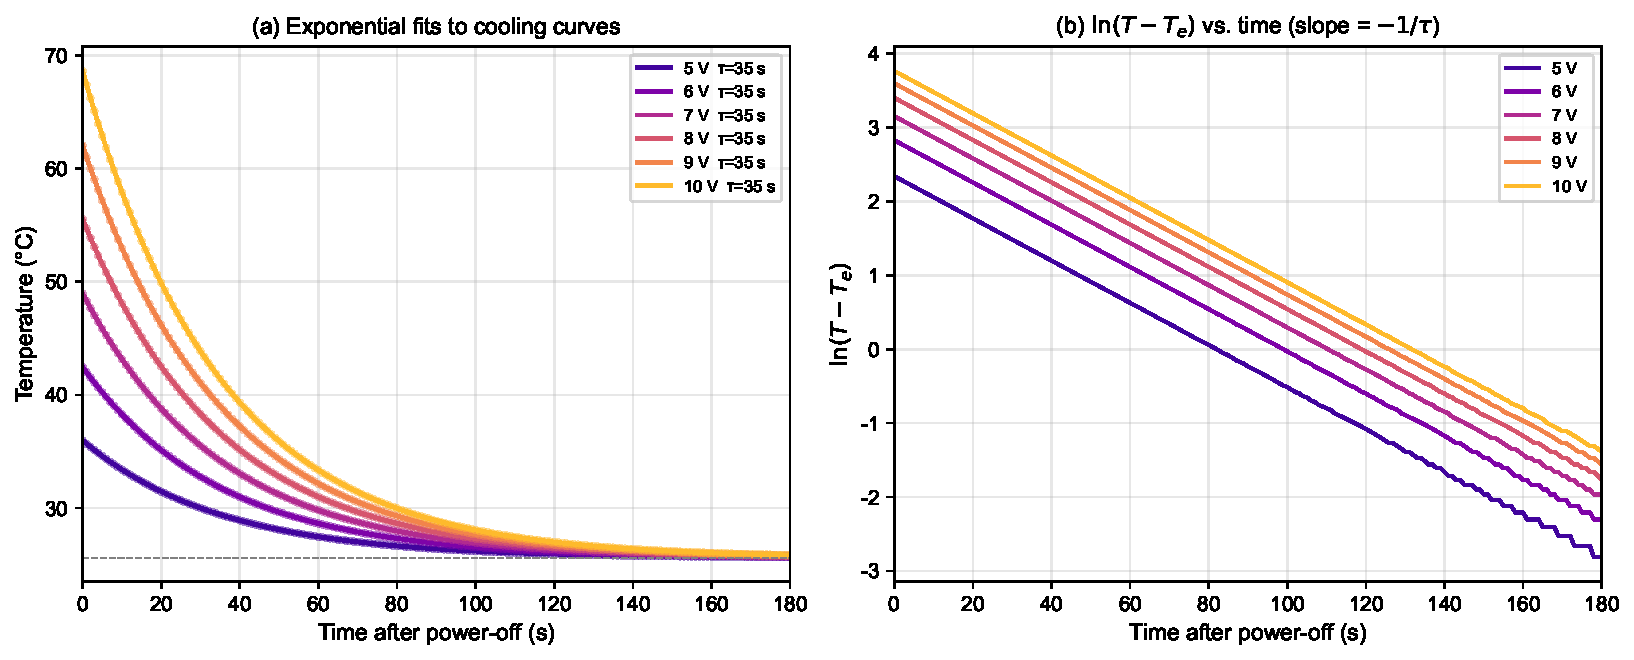
\includegraphics[width=0.48\textwidth]{fig_cooling_fit.pdf}\hfill
  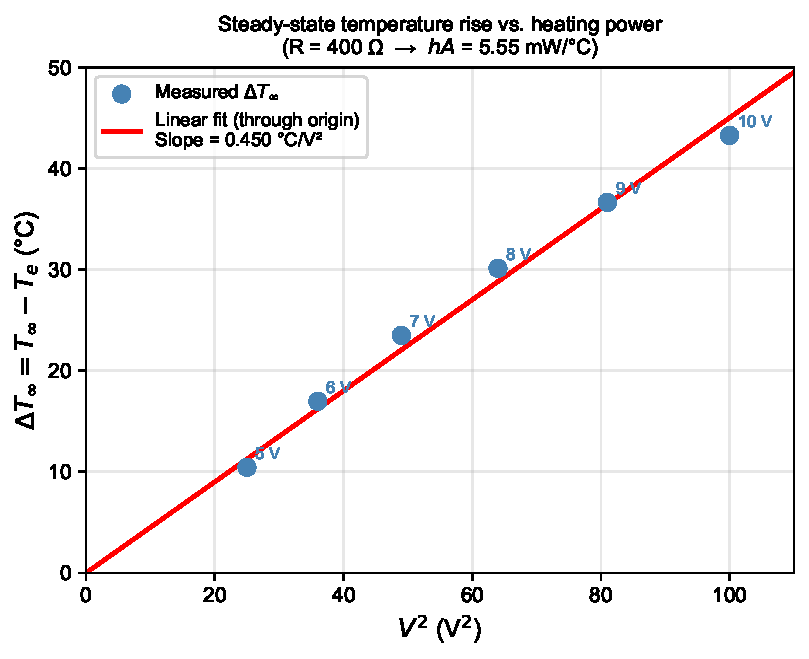
\includegraphics[width=0.48\textwidth]{fig_steady_state.pdf}
  \caption{左：降温曲线指数拟合及$\ln(T-T_e)$–时间关系（斜率$=-1/\tau$）；右：稳态温差$\Delta T_\infty$与$V^2$的线性关系，斜率为$1/(RhA)$。}
  \label{fig:ssfit}
\end{figure*}

表\,\ref{tab:heat}汇总了六组电压下的稳态温差及由此估算的$hA$值。各组结果相互吻合，验证了模型自洽性。

\begin{table}[H]
\centering
\caption{不同加热电压下的稳态温差与换热参数}
\label{tab:heat}
\begin{tabularx}{\columnwidth}{YYYY}
\toprule
$V$ (V) & $Q$ (mW) & $\Delta T_\infty$ (°C) & $hA$ (mW/°C) \\
\midrule
5  & 62.5  & 10.4 & 5.99 \\
6  & 90.0  & 17.0 & 5.30 \\
7  & 122.5 & 23.5 & 5.21 \\
8  & 160.0 & 30.1 & 5.31 \\
9  & 202.5 & 36.7 & 5.52 \\
10 & 250.0 & 43.3 & 5.78 \\
\midrule
\multicolumn{3}{l}{平均} & 5.52 \\
\bottomrule
\end{tabularx}
\end{table}

\subsection{PID调参实验}

教师指定的四个设定温度依次为$\SI{30}{\degreeCelsius}\to\SI{50}{\degreeCelsius}\to\SI{60}{\degreeCelsius}\to\SI{40}{\degreeCelsius}$。分别使用四组PID参数进行控温实验，参数及控温效果如表\,\ref{tab:pid}所示。

\begin{table}[H]
\centering
\caption{四组PID参数及控温效果评估}
\label{tab:pid}
\begin{tabularx}{\columnwidth}{cYYYY}
\toprule
组别 & $K_c$ & $T_i$ & $T_d$ & 评价 \\
\midrule
1 & 20 & 0.008 & 0.01  & \textbf{最优} \\
2 & 20 & 0.03  & 0.001 & 较差 \\
3 & 30 & 0.008 & 0.001 & 一般 \\
4 & 20 & 0.008 & 0.001 & 一般 \\
\bottomrule
\end{tabularx}
\end{table}

\subsection{设定温度$T_1=\SI{48.2}{\degreeCelsius}$调参实验}

以$T_1=(T_{\max}+T_e)/2=\SI{48.2}{\degreeCelsius}$为设定温度，分别使用四组PID参数从室温开始控温，观测升温过程及稳态效果，结果如图\,\ref{fig:img05}--\ref{fig:img08}所示。

第一组参数$(K_c=20,\;T_i=0.008,\;T_d=0.01)$的控温曲线如图\,\ref{fig:img05}所示。实际温度从室温快速上升并平稳趋近设定值$\SI{48.2}{\degreeCelsius}$，稳态温度约$\SI{48.1}{\degreeCelsius}$，几乎无超调，稳态波动极小，为四组中表现最优。

\begin{figure}[H]
  \centering
  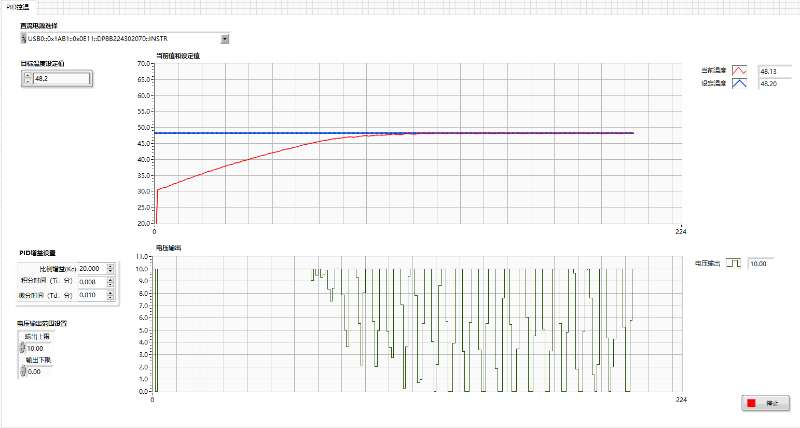
\includegraphics[width=0.95\columnwidth]{IMG_05.jpg}
  \caption{第一组参数$T_1=\SI{48.2}{\degreeCelsius}$控温曲线（\textbf{最优}）}
  \label{fig:img05}
\end{figure}

第二组参数$(K_c=20,\;T_i=0.03,\;T_d=0.001)$如图\,\ref{fig:img06}所示。$T_i$增大使积分作用减弱，温度上升较慢，稳态温度约$\SI{48.0}{\degreeCelsius}$，存在一定稳态误差，到达设定值的时间明显长于第一组。

\begin{figure}[H]
  \centering
  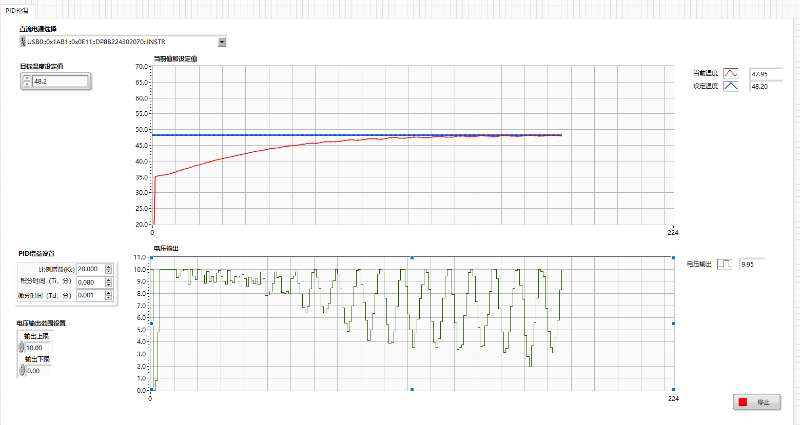
\includegraphics[width=0.95\columnwidth]{IMG_06.jpg}
  \caption{第二组参数$T_1=\SI{48.2}{\degreeCelsius}$控温曲线}
  \label{fig:img06}
\end{figure}

第三组参数$(K_c=30,\;T_i=0.008,\;T_d=0.001)$如图\,\ref{fig:img07}所示。$K_c$增大至30加快了响应，但$T_d$过小导致微分抑制不足，温度在设定值附近出现可见的振荡波动，稳态温度约$\SI{48.1}{\degreeCelsius}$。

\begin{figure}[H]
  \centering
  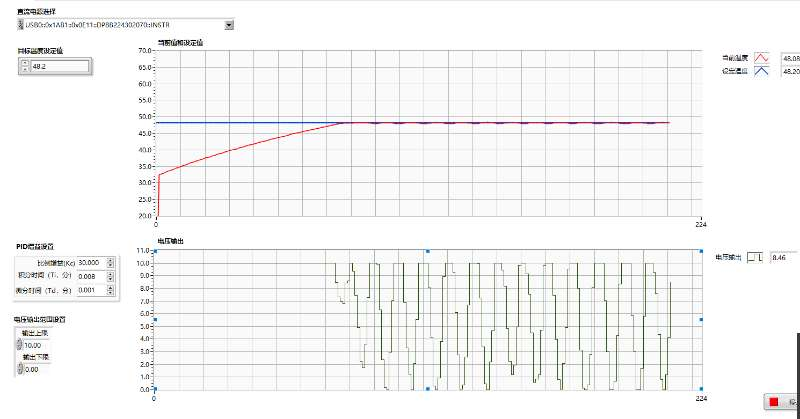
\includegraphics[width=0.95\columnwidth]{IMG_07.jpg}
  \caption{第三组参数$T_1=\SI{48.2}{\degreeCelsius}$控温曲线}
  \label{fig:img07}
\end{figure}

第四组参数$(K_c=20,\;T_i=0.008,\;T_d=0.001)$如图\,\ref{fig:img08}所示。与第一组仅$T_d$不同，微分"刹车"减弱后温度在趋近设定值时出现小幅振荡，稳态温度约$\SI{48.1}{\degreeCelsius}$，稳态波动略大于第一组。

\begin{figure}[H]
  \centering
  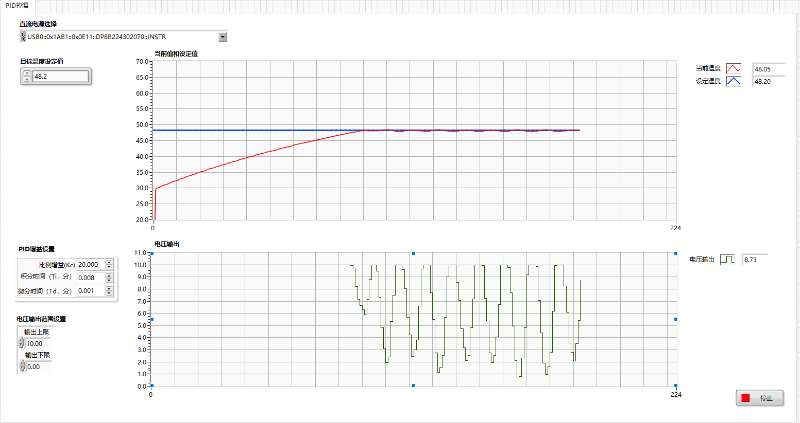
\includegraphics[width=0.95\columnwidth]{IMG_08.jpg}
  \caption{第四组参数$T_1=\SI{48.2}{\degreeCelsius}$控温曲线}
  \label{fig:img08}
\end{figure}

\subsection{四设定温度控温实验}

根据教师指定的设定温度$\SI{30}{\degreeCelsius}\to\SI{50}{\degreeCelsius}\to\SI{60}{\degreeCelsius}\to\SI{40}{\degreeCelsius}$，使用上述四组参数分别进行控温实验。

\subsubsection{第一组参数}

第一组参数$(K_c=20,\;T_i=0.008,\;T_d=0.01)$表现最优，其在四个设定温度段的控温曲线如图\,\ref{fig:img01}所示。上方曲线为温度响应曲线（红色为实际温度，蓝色为设定温度），下方曲线为对应的控制电压输出。可以看出实际温度能较好地跟踪设定温度，在各阶跃变化处超调量较小、稳态波动幅度可控，整体控温效果优于其他三组。

\begin{figure}[H]
  \centering
  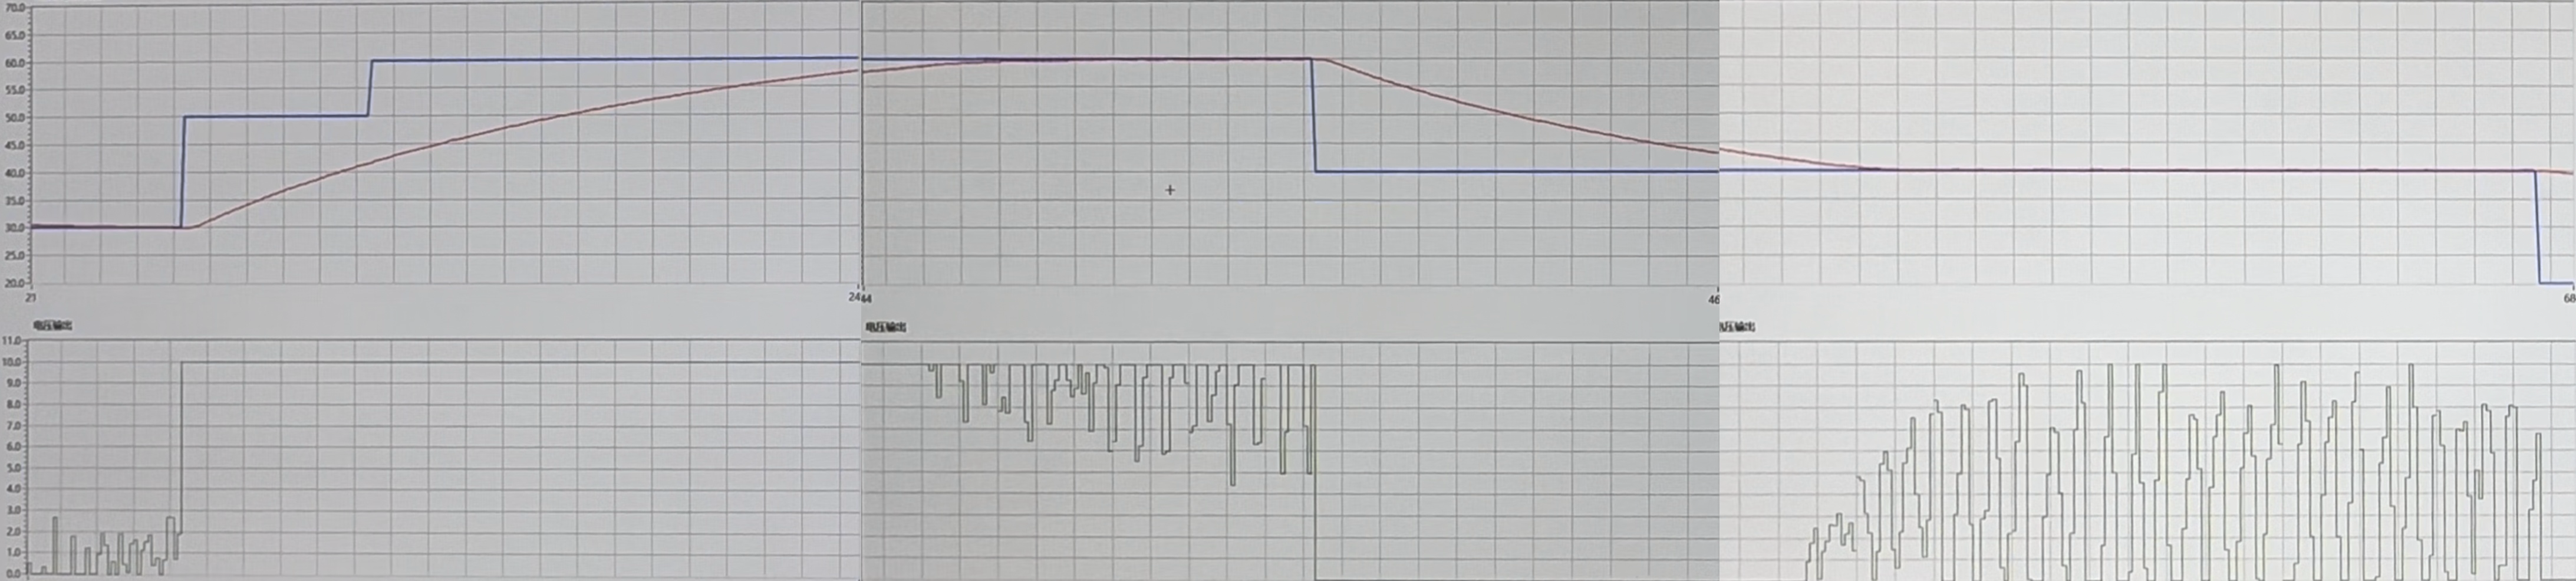
\includegraphics[width=0.95\columnwidth]{IMG_01.png}
  \caption{第一组PID参数$(K_c\!=\!20,\;T_i\!=\!0.008,\;T_d\!=\!0.01)$控温曲线}
  \label{fig:img01}
\end{figure}

\subsubsection{第二组参数}

第二组参数$(K_c=20,\;T_i=0.03,\;T_d=0.001)$的控温曲线如图\,\ref{fig:img02}所示。与第一组相比，$T_i$从0.008增大至0.03，积分项$(K_c/T_i)$的作用减弱，消除稳态误差的速度变慢，可见实际温度到达设定值存在明显滞后；同时$T_d$减小为0.001使微分"刹车"减弱，控温效果较差。

\begin{figure}[H]
  \centering
  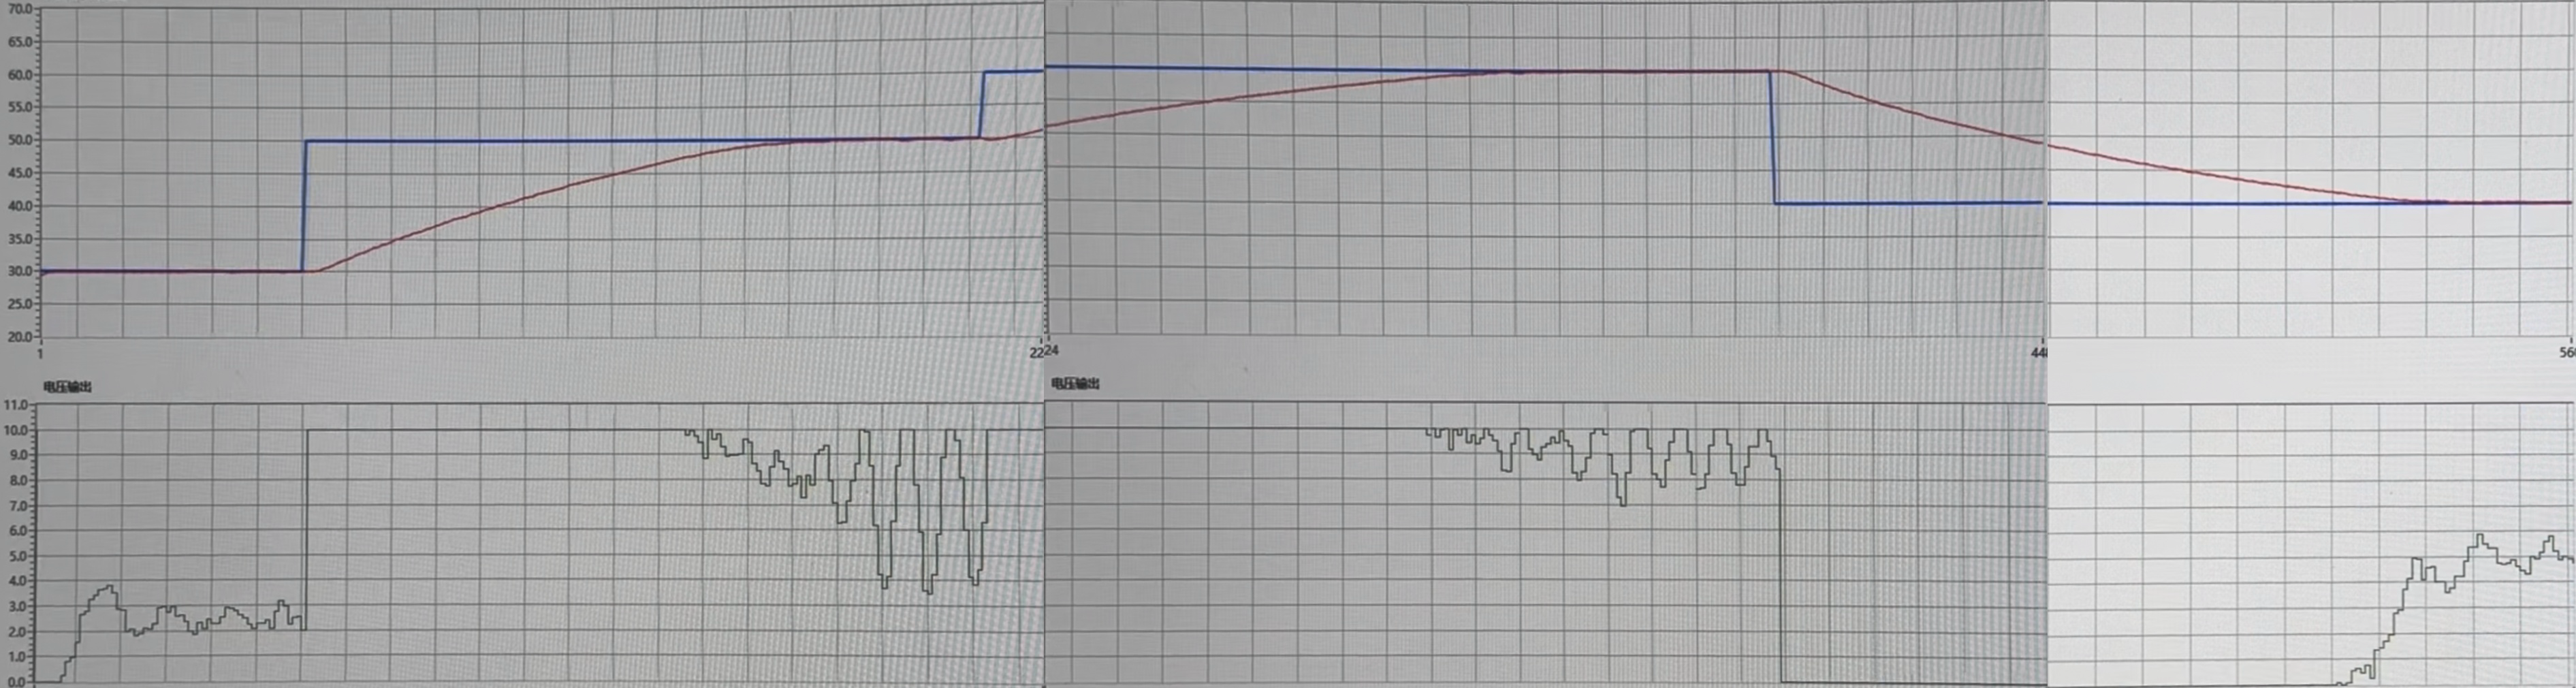
\includegraphics[width=0.95\columnwidth]{IMG_02.png}
  \caption{第二组PID参数$(K_c\!=\!20,\;T_i\!=\!0.03,\;T_d\!=\!0.001)$控温曲线}
  \label{fig:img02}
\end{figure}

\subsubsection{第三组参数}

第三组参数$(K_c=30,\;T_i=0.008,\;T_d=0.001)$的控温曲线如图\,\ref{fig:img03}所示。$K_c$增大至30使比例作用增强、响应加快，但同时$T_d$仅为0.001导致微分抑制不足，两者叠加使系统出现较明显的振荡和超调，电压输出波动也更为剧烈。

\begin{figure}[H]
  \centering
  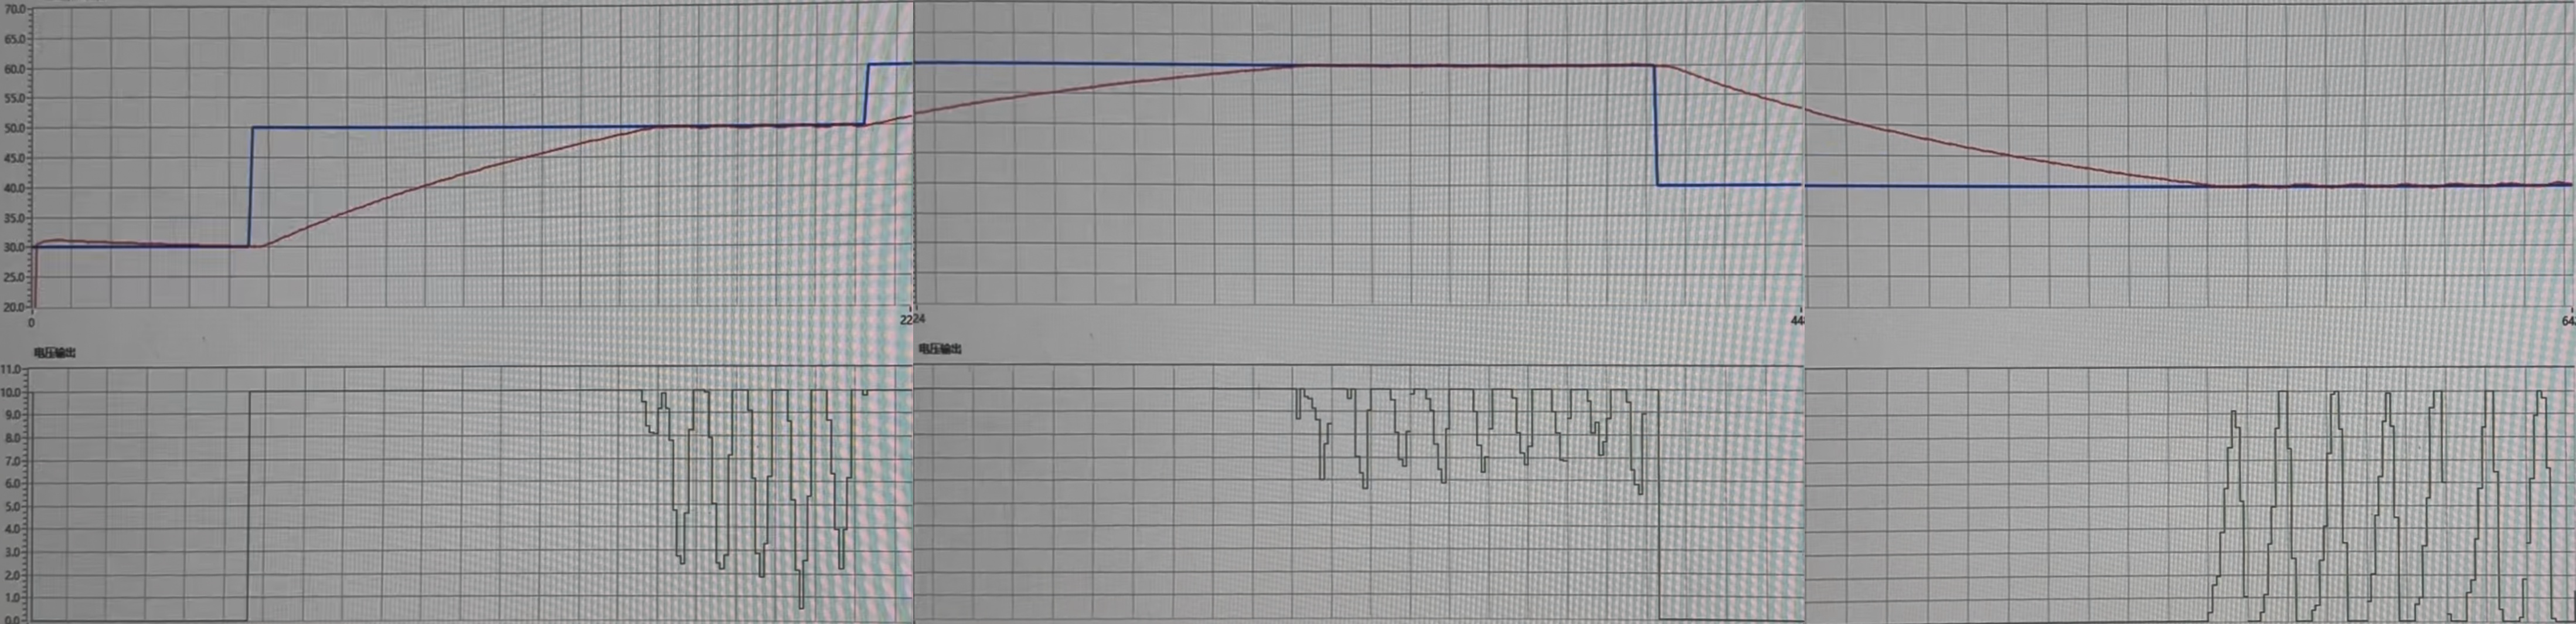
\includegraphics[width=0.95\columnwidth]{IMG_03.png}
  \caption{第三组PID参数$(K_c\!=\!30,\;T_i\!=\!0.008,\;T_d\!=\!0.001)$控温曲线}
  \label{fig:img03}
\end{figure}

\subsubsection{第四组参数}

第四组参数$(K_c=20,\;T_i=0.008,\;T_d=0.001)$的控温曲线如图\,\ref{fig:img04}所示。该组与第一组仅$T_d$不同（0.001 vs 0.01），可以单独考察微分项的影响：$T_d$减小一个量级后微分"刹车"作用显著减弱，在设定值阶跃变化时超调增大，稳态时温度波动幅度也有所增大，电压输出呈现更密集的振荡。

\begin{figure}[H]
  \centering
  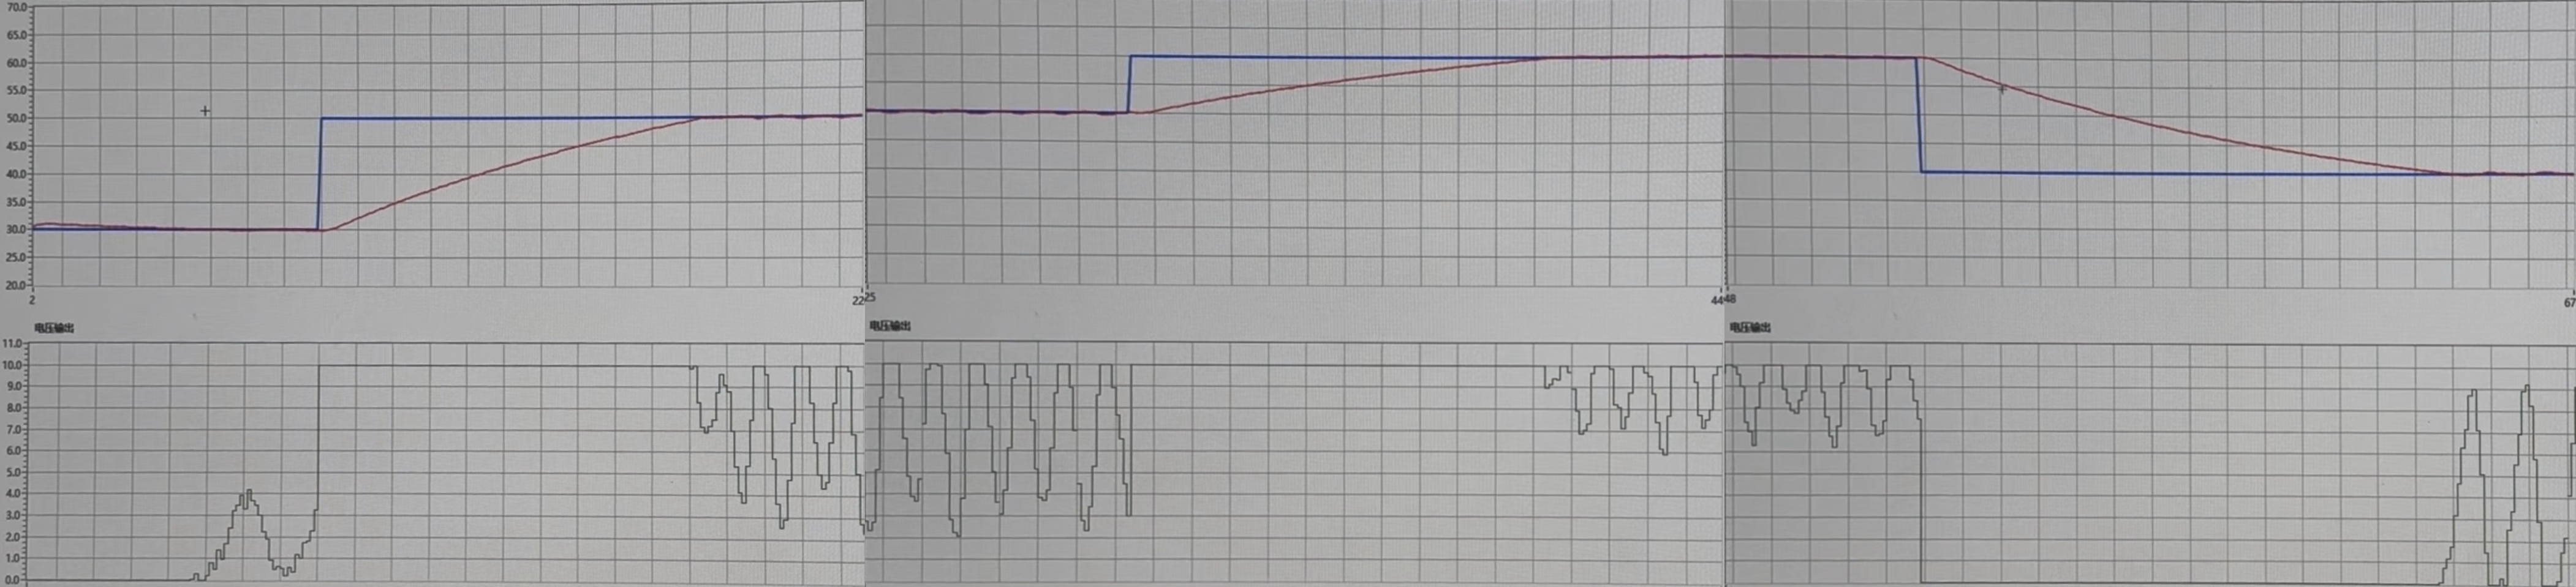
\includegraphics[width=0.95\columnwidth]{IMG_04.png}
  \caption{第四组PID参数$(K_c\!=\!20,\;T_i\!=\!0.008,\;T_d\!=\!0.001)$控温曲线}
  \label{fig:img04}
\end{figure}

\subsection{参数对比分析}

综合四组实验结果，对PID参数的影响规律分析如下：

\begin{enumerate}
  \item \textbf{比例增益$K_c$}：对比第一组（$K_c=20$）和第三组（$K_c=30$），增大$K_c$加快了响应速度，但同时加剧了振荡和超调。在$K_c=20$时系统已有较好的响应速度，进一步增大反而降低了稳定性。

  \item \textbf{积分时间$T_i$}：对比第一组（$T_i=0.008$）和第二组（$T_i=0.03$），较大的$T_i$使积分作用减弱，消除稳态误差的速度变慢，温度到达设定值的时间延长。

  \item \textbf{微分时间$T_d$}：对比第一组（$T_d=0.01$）和第四组（$T_d=0.001$），较大的$T_d$提供了更强的"刹车"效果，有效抑制超调和振荡。$T_d=0.01$时系统在阶跃响应中几乎无超调，而$T_d=0.001$时出现明显超调。
\end{enumerate}

因此，第一组参数$(K_c=20,\;T_i=0.008,\;T_d=0.01)$在响应速度、超调量和稳态精度之间取得了最佳平衡，为本实验条件下的最优PID参数。

%%%%%%%%%%%%%%%%%%%%%%%%%%%%%%%%%%%%%%%%%%%%%%%%%%%%%%%%%%%%
\section{讨论与分析}

\begin{enumerate}
  \item \textbf{P、I、D三个参数分别对控温效果有什么影响？}\\[0.3em]
  比例增益$K_p$决定系统对当前偏差的响应强度，增大$K_p$可加快响应但过大会导致振荡；积分项$1/T_i$累积历史偏差以消除稳态误差，但过强的积分作用会引起积分饱和和超调；微分项$T_d$根据偏差变化率提前"刹车"，抑制超调和振荡，但过大会放大测量噪声。三者需协调配合才能获得良好的控温效果。

  \item \textbf{为何第一组参数表现最优？}\\[0.3em]
  第一组参数$T_d=0.01$较大，提供了充足的微分"刹车"能力，有效抑制了阶跃设定值变化时的超调；$T_i=0.008$保证了积分项能快速消除稳态误差；$K_c=20$在响应速度和稳定性之间取得平衡。综合三项作用，该参数组合使系统在各温度段均表现出快速响应、低超调和小稳态波动的良好特性。
\end{enumerate}

%%%%%%%%%%%%%%%%%%%%%%%%%%%%%%%%%%%%%%%%%%%%%%%%%%%%%%%%%%%%
\clearpage
\onecolumn
\section*{参考文献}

\begin{enumerate}[label={[\arabic*]}]
  \item Morris Driels~著, 金爱娟, 李少龙, 李航天~译. 线性控制系统工程[M]. 北京: 清华大学出版社, 2005.
  \item 吴麒, 王诗宓~编. 自动控制原理（第二版）（上）[M]. 北京: 清华大学出版社, 2006.
  \item Ogata K. Modern Control Engineering[M]. 5th ed. Pearson, 2010.
\end{enumerate}

\clearpage

\section*{教师签名页}
\begin{figure}[htbp]
  \centering
  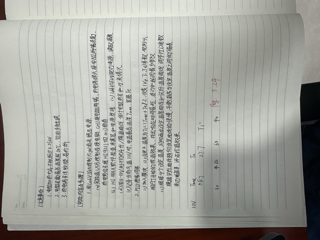
\includegraphics[width=\textwidth,height=0.85\textheight,keepaspectratio]{Sign.png}
\end{figure}

\end{document}
